\documentclass[assignment = 0]{homework}

\usepackage{caption, subcaption, pdfpages, float}
\usepackage{graphics, wrapfig, pgf, graphicx}
\graphicspath{{../}}


% pacotes para importar código
\usepackage{caption, booktabs}
\usepackage[section, newfloat]{minted}
\definecolor{sepia}{RGB}{252,246,226}
\setminted{
    bgcolor = sepia,
    style   = pastie,
    frame   = leftline,
    autogobble,
    samepage,
    python3,
}
\setmintedinline{
    bgcolor={}
}

% ambientes de códigos de Python
\newmintedfile[pyinclude]{python}{}
\newmintinline[pyline]{python}{}
\newcommand{\pyref}[2]{\href{#1}{\texttt{#2}}}

\SetupFloatingEnvironment{listing}{name=Código}

\usepackage{csquotes}
\usepackage[style=authortitle-ibid,backend=biber]{biblatex}
\bibliography{referencias}
\usepackage[noabbrev, nameinlink, brazilian]{cleveref}
\usepackage[section]{placeins}

\begin{document}

    \section{Introdução}

O objetivo deste trabalho é de realizar processamentos básicos de imagem e se familiarizar com Python e suas ferramentas. Pensando nisso, o programa desenvolvido utiliza a biblioteca OpenCV para leitura, codificação e decodificação de imagens PNG e usa Numpy para tratamento vetorizado da imagem.

Todos os processamentos serão aplicados nas mesmas imagens da especificação do trabalho e uma imagem colorida, apresentada na \cref{fig:color}.

\begin{figure}[H]
    \centering
    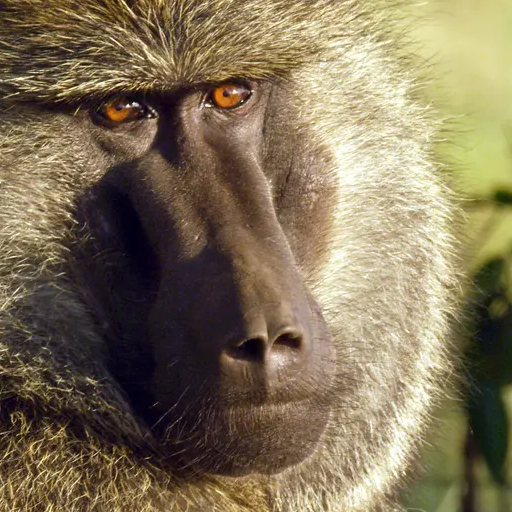
\includegraphics[width=6cm]{imagens/color.png}

    \caption{Imagem colorida usada como comparação dos resultados dos processamentos.}
    \label{fig:color}
\end{figure}

\section{O Programa}

\subsection{Código Fonte}

O programa foi desenvolvido em 4 arquivos separados:

\begin{description}
    \item[main.py] É o corpo do programa, resposável por processar os comandos e opções da linha de comando.

    \item[inout.py] Funções que tratam da entrada e saída do programa, como leitura e escritas de arquivos de imagem e também da apresentação da imagem em uma janela gráfica.

    \item[lib.py] Funções de tranformação da imagem, como ajute de brilho e acesso do plano de bits.

    \item[tipos.py] Definição dos tipos para tipagem estática (apenas o protocolo \autocite{ref:pep544} \pyline{Image}).
\end{description}

A tipagem estática é aplicada para facilitar o desenvolvimento e a leitura do código, mas ela limita a execução em Python para as versões 3.7 ou superior \autocite{ref:pep563}.

Todas as figuras base utilizadas neste relatório podem ser encontradas na pasta \texttt{imagens}. A \cref{fig:color}, por exemplo, está em \texttt{imagens/color.png}.

\subsection{Execução}

A execução deve ser feita através do interpretador de Python 3.7+. A única entrada obrigatória é o caminho para a imagem PNG que será processada. As entradas seguintes serão tratadas como comandos de processamento da imagem. Ao final da execução, a imagem resultante será exibida na tela. Por exemplo, o comando abaixo exibe na tela a \cref{fig:execucao}.

\begin{minted}{bash}
    $ python3.8 main.py imagens/color.png monocromatico plano.bit 6 negativo \
        mosaico padrao.txt
\end{minted}

\begin{figure}[H]
    \centering
    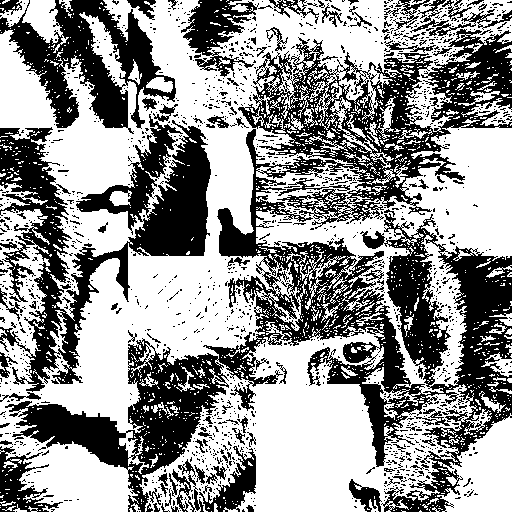
\includegraphics[width=6cm]{resultados/execucao.png}

    \caption{Aplicação de alguns processamentos na \cref{fig:color}.}
    \label{fig:execucao}
\end{figure}

Além das entradas posicionais, existem dois argumentos opicionais. Com \mintinline{bash}{--output}, ou \mintinline{bash}{-o}, é possível gravar o resultado em um arquivo PNG em vez de exibir na tela. O comando abaixo resulta na mesma imagem da \cref{fig:execucao}, mas guarda em um arquivo \texttt{out.png}, sem exibir na tela.

\begin{minted}{bash}
    $ python3.8 main.py imagens/color.png -o out.png monocromatico plano.bit 6 \
        negativo mosaico padrao.txt
\end{minted}

Se é desejável tanto a exibição da imagem quanto o salvamento no arquivo, o argumento \mintinline{bash}{--force-show} ou \mintinline{bash}{-f} pode ser usado.

\subsection{Comandos Entendidos}

O programa entende dez comandos distintos, apresentados abaixo, que podem ser repetidos quantas vezes forem necessárias. Os comandos são executados na ordem em que aparecem na linha de comando.

Todos os comandos abaixos devem ser usados da mesma forma como aparecem aqui, em letras minúsculas, sem acentos e com ponto onde aparecer abaixo. Os nomes em letras maiúsculas são os argumentos daquele comando, que devem aparecem após o nome do comando (a maioria deles não tem argumentos).

\begin{description}
    \item[\texttt{monocromatico}] Transforma a imagem para monocromática, em escala de cinza. Só faz diferente para entradas coloridas.

    \item[\texttt{negativo}] Inverte a intensidade de cada pixel da imagem, em todos os canais de cores.

    \item[\texttt{esp.verical}] Faz o espelhamento vertical da imagem.

    \item[\texttt{conv.intervalo}] Converte o intervalo de intensidades para [100, 200].

    \item[\texttt{inverte.pares}] Inverte a direção dos píxeis das linhas pares da imagem.

    \item[\texttt{reflexao}] Faz a reflexão das linhas superiores.

    \item[\texttt{aj.brilho GAMA}] Aplica um ajuste de brilho com fator \texttt{GAMA}.

    \item[\texttt{plano.bit M}] Extrai o plano de bit de ordem \texttt{M} para ordens em [0, 8).

    \item[\texttt{combina IMAGEM ALPHA}] Faz a combinação com outra imagem PNG no arquivo \texttt{IMAGEM} por média ponderada com um fator de peso \texttt{ALPHA}.

    \item[\texttt{mosaico ORDENACAO}] Contrói um mosaico da imagem a partir de nova ordem dos blocos descrita no arquivo \texttt{ORDENACAO} (detalhes na \cref{sec:mosaico}).
\end{description}


    \section{Implementação}

Toda a parte de processamento de imagem se encontra no código fonte \texttt{lib.py}. Cada subseção mostra no trecho de código qual função nesse arquivo se encontra a implementação da operação. Os trechos apresentados refletem o código no arquivo, mas sem detalhes como cópias de \textit{buffer} e tipagem estática.

Quando possível, a função equivalente do OpenCV também será apresentada, já que as acelerações de GPU podem ser mais facilmente acessadas usando \pyline{cv2.cuda} em vez de apenas \pyline{cv2} \autocite{ref:cvcuda}. Entretanto, as operações foram implementadas apenas com Numpy neste trabalho, visando a familiarização com técnicas de vetorização.

Assuma que as bibliotecas são importadas como:

\begin{minted}{python}
    import numpy as np
    import cv2
\end{minted}

\subsection{Conversão para Monocromático}

A transformação para escala de cinza é feita através da média dos três canais de cores, truncada para inteiro. A matriz resultante é então repetida novamente para os três canais, para que a operação possa ser repetida sem erros de execução do programa.

\begin{listing}[h]
    \caption{Comando \texttt{monocromatico}}

    \begin{minted}{python}
        def grayscale(imagem):
            gray = np.mean(imagem, axis=2).astype(np.uint8)
            return np.stack([gray, gray, gray], axis=2)
    \end{minted}
\end{listing}

\begin{figure}
    \centering
    \begin{subfigure}{0.45\textwidth}
        \centering
        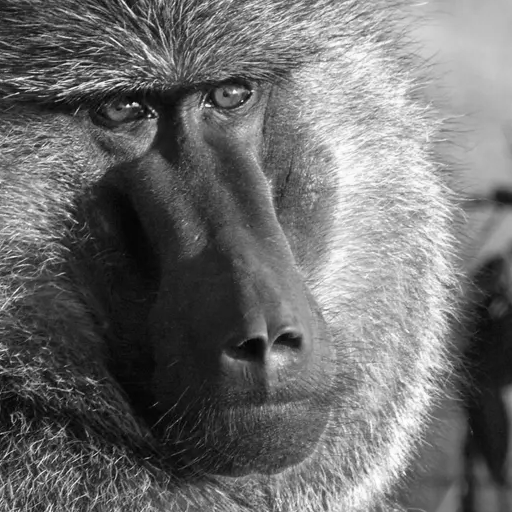
\includegraphics[width=6cm]{resultados/colormono.png}
        \caption{\texttt{imagens/color.png}}
    \end{subfigure}%
    \begin{subfigure}{0.45\textwidth}
        \centering
        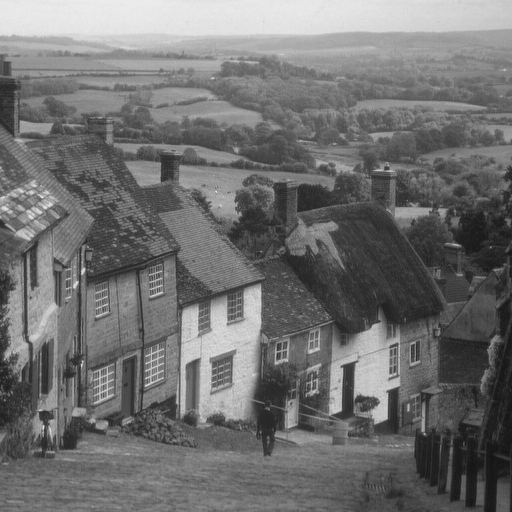
\includegraphics[width=6cm]{resultados/citymono.png}
        \caption{\texttt{imagens/city.png}}
    \end{subfigure}

    \caption{Mudaça para escala de cinza.}
\end{figure}

Em vez de \pyline{np.mean(imagem, ...)}, a conversão poderia ser implementado também com \pyline{cv2.cvtColor(image, cv2.COLOR_BGR2GRAY)} \autocite{ref:cvtcolor}.

\subsection{Negativo da Imagem}

Para essa conversão basta fazer ~\pyline{255 - intensidade}~ para cada píxel. Como 255 também é o maior valor de um \textit{byte}, basta também inverter todos os bits da imagem.

\begin{figure}[H]
    \centering
    \begin{subfigure}{0.45\textwidth}
        \centering
        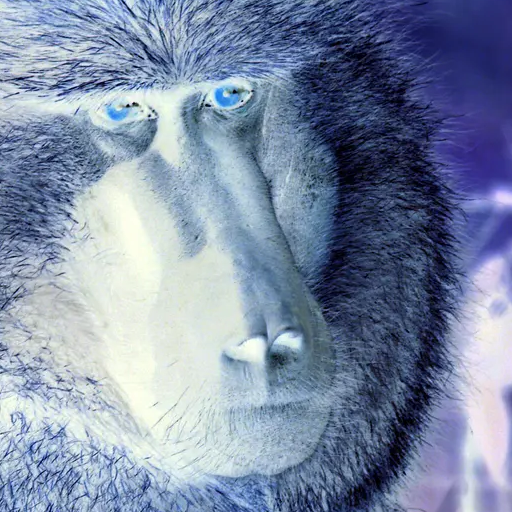
\includegraphics[width=6cm]{resultados/colorneg.png}
        \caption{\texttt{imagens/color.png}}
    \end{subfigure}%
    \begin{subfigure}{0.45\textwidth}
        \centering
        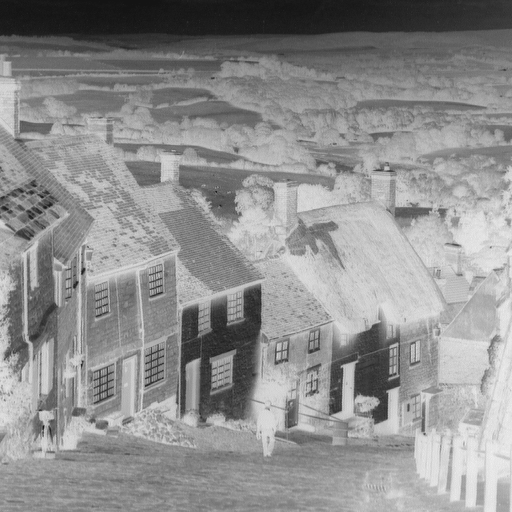
\includegraphics[width=6cm]{resultados/cityneg.png}
        \caption{\texttt{imagens/city.png}}
    \end{subfigure}

    \caption{Imagem com intensidade invertida.}
\end{figure}

\begin{listing}[H]
    \caption{Comando \texttt{negativo}}

    \begin{minted}{python}
        def negativo(imagem):
            return ~imagem
    \end{minted}
\end{listing}

Em vez de usar o \textit{not} do Numpy, existe também a função \pyline{cv2.bitwise_not(imagem)} \autocite{ref:bitwise_not}.

\subsection{Espelhamento Vertical}

\begin{listing}[h]
    \caption{Comando \texttt{esp.vertical}}

    \begin{minted}{python}
        def espelhamento_vertical(imagem):
            return imagem[::-1]
    \end{minted}
\end{listing}

\begin{figure}[h]
    \centering
    \begin{subfigure}{0.45\textwidth}
        \centering
        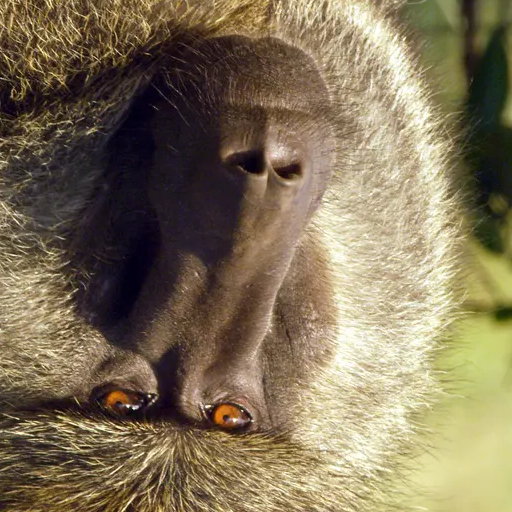
\includegraphics[width=6cm]{resultados/colorflip.png}
        \caption{\texttt{imagens/color.png}}
    \end{subfigure}%
    \begin{subfigure}{0.45\textwidth}
        \centering
        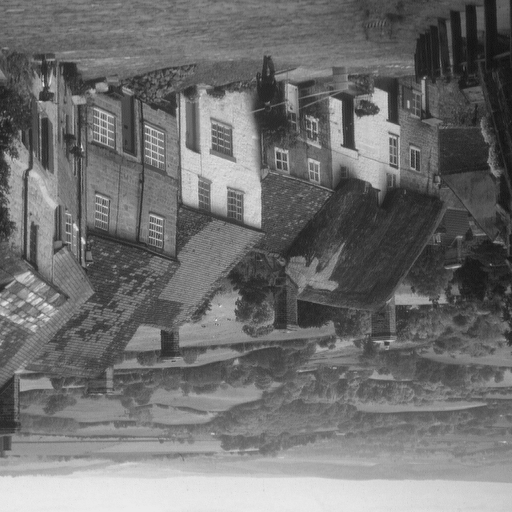
\includegraphics[width=6cm]{resultados/cityflip.png}
        \caption{\texttt{imagens/city.png}}
    \end{subfigure}

    \caption{Espelhamento vertical.}
\end{figure}

Pode ser implementado também com \pyline{cv2.flip(imagem, 0)} \autocite{ref:flip}.

\subsection{Conversão de Intervalo}

Converte o intervalo de intensidade da imagem de [0, 255] para [100, 200] linearmente.

\begin{listing}[h]
    \caption{Comando \texttt{conv.intervalo}}

    \begin{minted}{python}
        def converter_intervalo(imagem):
            zmin, zmax = np.min(imagem), np.max(imagem)
            img = 100 * (image / 255) + 100
            return img.astype(np.uint8)
    \end{minted}
\end{listing}

\begin{figure}[!htb]
    \centering
    \begin{subfigure}{0.45\textwidth}
        \centering
        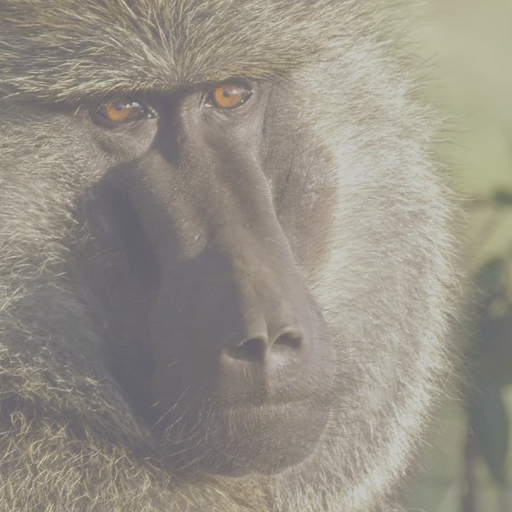
\includegraphics[width=6cm]{resultados/colorconv.png}
        \caption{\texttt{imagens/color.png}}
    \end{subfigure}%
    \begin{subfigure}{0.45\textwidth}
        \centering
        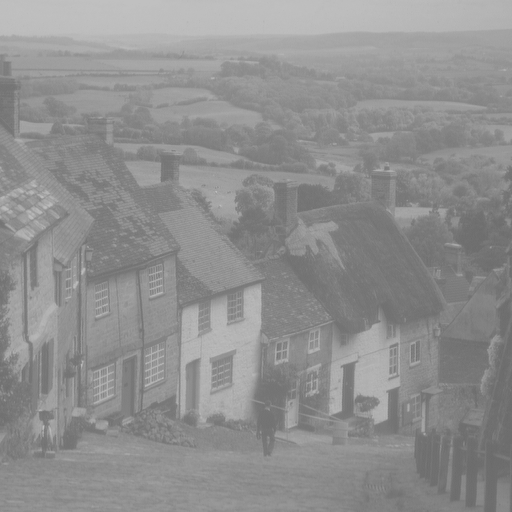
\includegraphics[width=6cm]{resultados/cityconv.png}
        \caption{\texttt{imagens/city.png}}
    \end{subfigure}

    \caption{Intervalo de intensidade convertido.}
\end{figure}

\subsection{Inversão das Linhas Pares}

Inverte todas as linhas pares horizontalmente.

\begin{figure}[h]
    \centering
    \begin{subfigure}{0.45\textwidth}
        \centering
        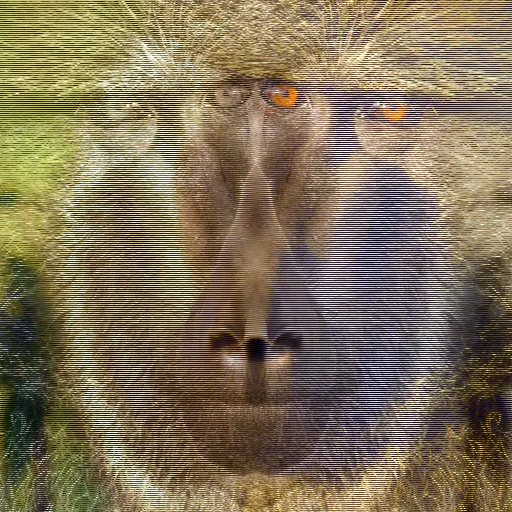
\includegraphics[width=6cm]{resultados/colorinvp.png}
        \caption{\texttt{imagens/color.png}}
    \end{subfigure}%
    \begin{subfigure}{0.45\textwidth}
        \centering
        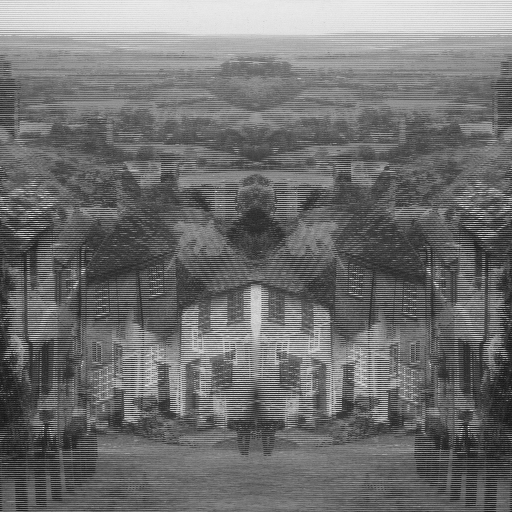
\includegraphics[width=6cm]{resultados/cityinvp.png}
        \caption{\texttt{imagens/city.png}}
    \end{subfigure}

    \caption{Linhas pares invertidas.}
\end{figure}

\begin{listing}[H]

    \begin{minted}{python}
        def inverte_linhas_pares(imagem):
            magem[::2] = image[::2,::-1]
            return imagem
    \end{minted}

    \caption{Comando \texttt{inverte.pares}}
\end{listing}

\subsection{Mosaico} \label{sec:mosaico}

\textcolor{red}{ORDENACAO? PADRAO? IMPL?}

\begin{minted}{text}
    $ python main.py imagens/baboon.png mosaico padrao.txt
\end{minted}

\begin{figure}[H]
    \centering
    \begin{subfigure}{0.45\textwidth}
        \centering
        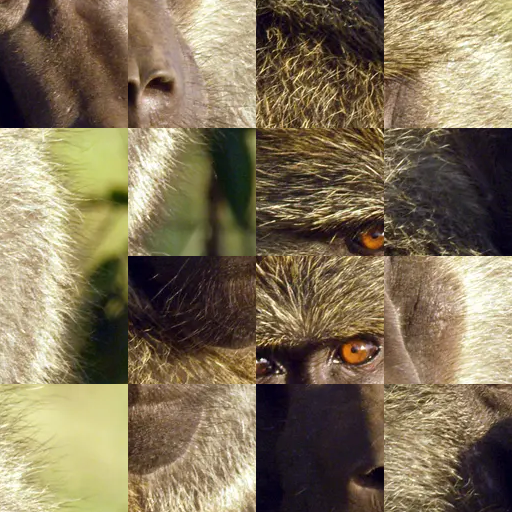
\includegraphics[width=6cm]{resultados/colormsc.png}
        \caption{\texttt{imagens/color.png}}
    \end{subfigure}%
    \begin{subfigure}{0.45\textwidth}
        \centering
        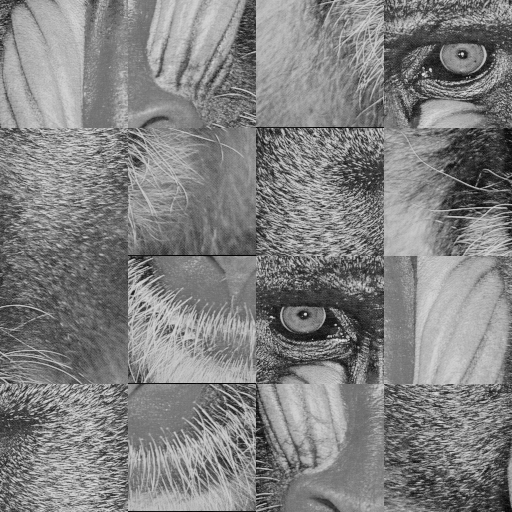
\includegraphics[width=6cm]{resultados/baboonmsc.png}
        \caption{\texttt{imagens/babooon.png}}
        \label{fig:res:10}
    \end{subfigure}

    \caption{Mosaico da imagem com \textcolor{red}{ALGUMA COISA}.}
\end{figure}

\begin{listing}[H]
    \begin{minted}{python}
        def mosaico(imagem, ordem):
            N, M = ordem.shape
            # split e flatten
            bloco = [
                bloco
                for lin in np.vsplit(imagem, N)
                for bloco in np.hsplit(lin, M)
            ]
            # accesso (em lista) e concatena
            imagem = np.concatenate([
                np.concatenate([bloco[i] for i in lin], axis=1)
                for lin in ordem
            ])
            return imagem
    \end{minted}

    \caption{Comando \texttt{mosaico ORDENACAO}}
\end{listing}



    \section{Resultados}

    Apesar de não ter nenhuma métrica de comparação das imagens, a análise visual permite dizer que o resultado foi satisfatório, isto é, as operações com as imagens obtiveram resultados próximos com o apresentado na especificação do trabalho. Em especial, as \crefrange{fig:res:1}{fig:res:10} ficaram muito similares às apresentadas no enunciado, com exceção talvez da \cref{fig:res:4}.

    Além disso, as funções puderam ser vetorizadas facilmente, no geral. A única exceção foi a o mosaico (\cref{sec:mosaico}), que foi implementado com alguns laços sobre os blocos da imagem.

\end{document}
